\begin{figure*}[t]
    \centering
    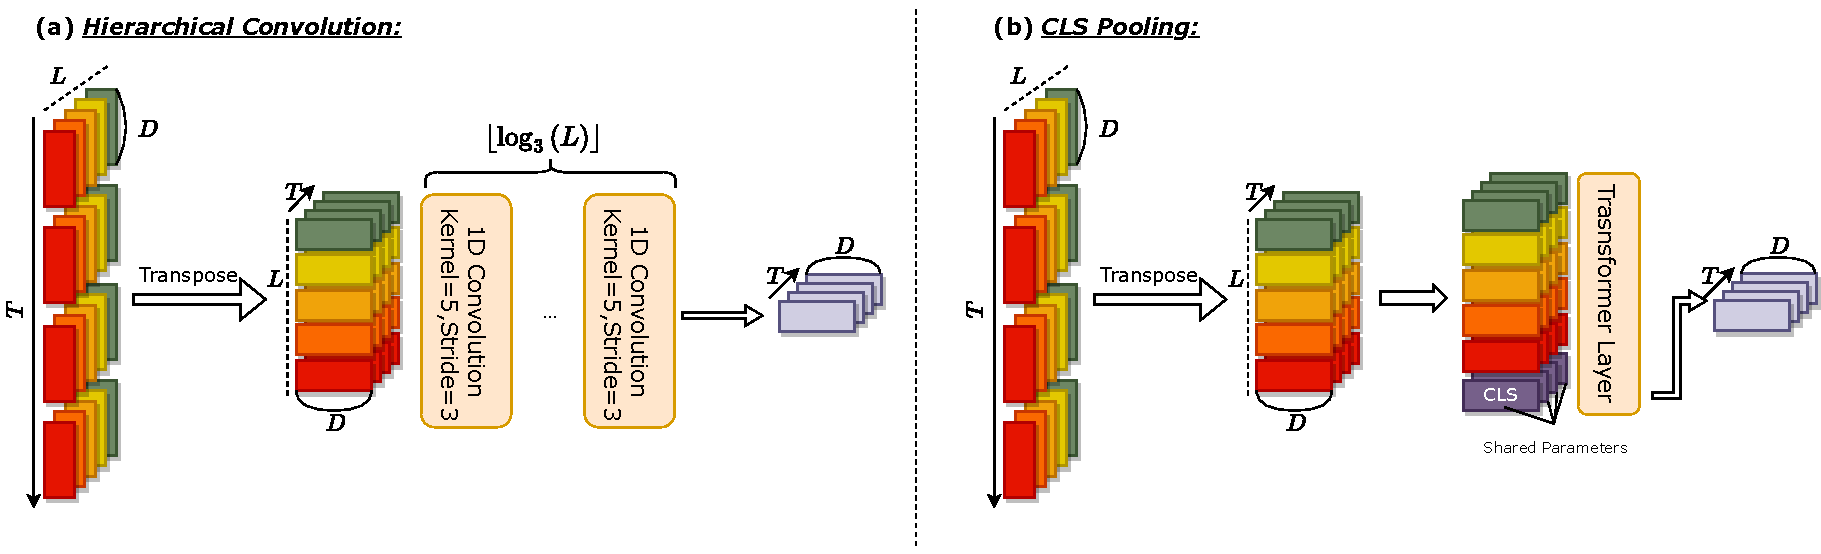
\includegraphics[width=\linewidth,trim={0cm 0.20cm 0cm 0},clip]{figs/SSL_Interface-ConvAndCLS.pdf}
    \caption{Proposed Interface designs. (a): Hierarchical Convolution is applied over the layer dimension of the upstream model hiddenstates. (b): A learnable CLS embedding is used for summarizing over layer dimension}
    \label{fig:interface_conv_cls}
    \vspace{-10pt}
\end{figure*}

\subsection{Interface Definition}

We formalize our proposed overall pipeline for utilizing self-supervised speech models as a general framework (as shown in Fig.~\ref{fig:framework}): \textbf{Upstream} $\rightarrow$ \textbf{Interface} $\rightarrow$ \textbf{Downstream}.
The \textbf{Upstream} model $\mathrm{U}\left(\cdot \right): \mathbb{R}^{T'} \mapsto \mathbb{R}^{L\times T\times D} $ stands for a pre-trained, self-supervised speech model which maps an utterance waveform ${x} \in \mathbb{R}^{T'}$ of length $T'$ to a hidden representation $\boldsymbol{h}$ which consists of $L$ representation layers each with a feature dimension of $D$.
\textbf{Interface} is a function that aggregates information over the layer dimension $L$ of the upstream output, $\mathrm{I}\left(\cdot \right): \mathbb{R}^{L\times T\times D} \mapsto \mathbb{R}^{ T\times D} $.
Finally, \textbf{Downstream} $\mathrm{D}\left(\cdot \right)$ takes $\boldsymbol{z} = \mathrm{I}\left( \boldsymbol{h} \right)$ as input and outputs predictions for a specific downstream task.
Under this general framework, the weighted sum can be viewed as a specific type of interface,
\begin{equation}
    \mathrm{I}_{\mathrm{WS}}\left( \boldsymbol{h}  \right)=\sum_{l}^{L}{w_l \cdot \boldsymbol{h}_l}
    \label{eq:weightedsum}
\end{equation}
where $\boldsymbol{w}$ is the per-layer weight vector, which is typically learned jointly with the downstream model weights.

% The weighted sum interface has the benefit of being able to aggregate information across all $L$ layers of the upstream model while being very lightweight with only $L$ learnable parameters.
The weighted sum interface has the benefit of being able to aggregate information across all $L$ upstream layers with only $L$ learnable parameters required.
% while being very lightweight with only $L$ learnable parameters.
On the other hand, we hypothesize that it has potential downsides: by directly summing layer representations dimension-wise, statistically independent features from different layers of the upstream model may "collide" with one another resulting in information loss.
As the number of layers in the upstream model increases, this problem can become more severe.
To further investigate this, we propose several alternative interface designs that attempt to avoid information collision across multiple upstream layers while remaining relatively lightweight and also keeping the output dimension roughly the same as the upstream model's dimension.

% \begin{figure}[h]
%     \centering
%     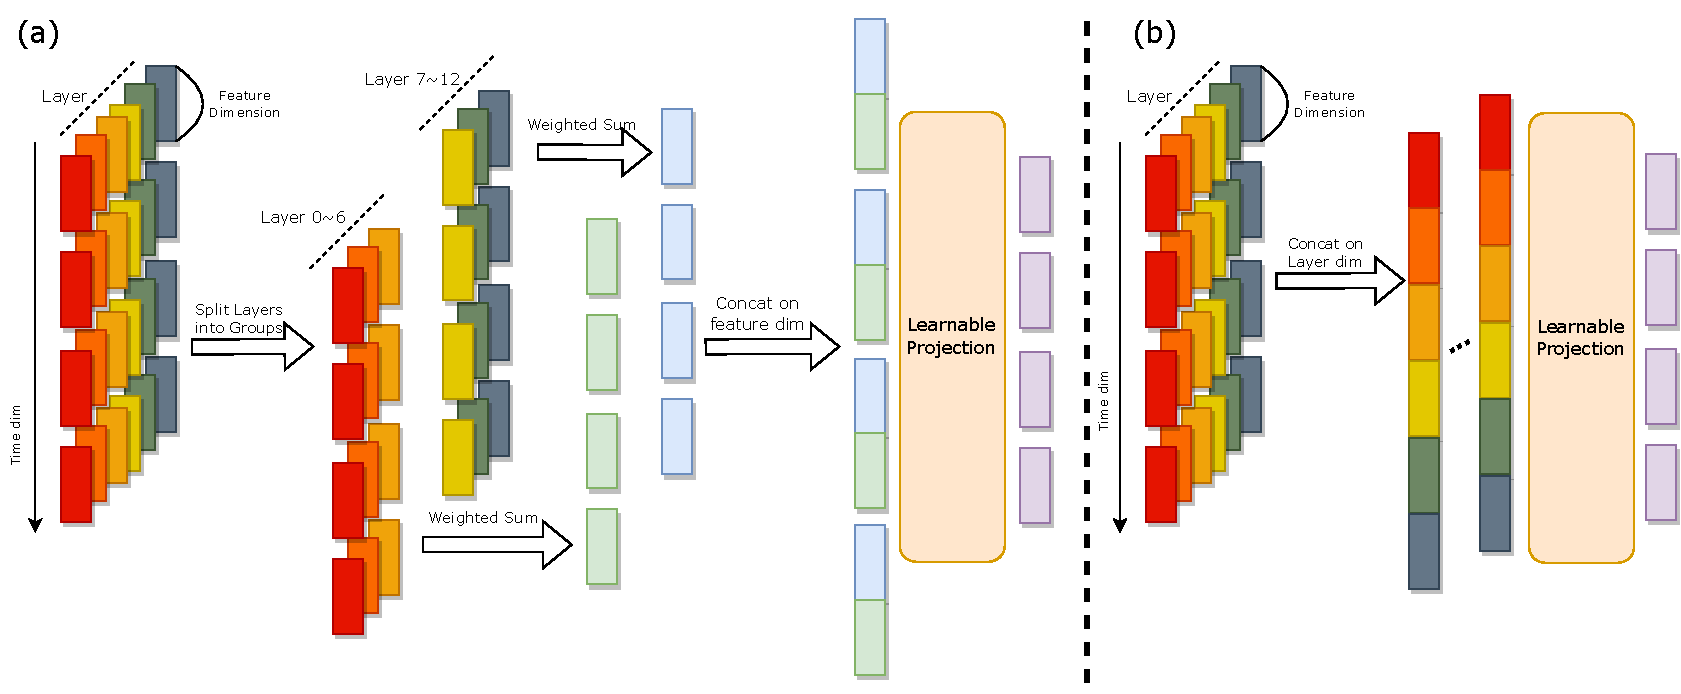
\includegraphics[width=\linewidth]{figs/interface_ab.pdf}
%     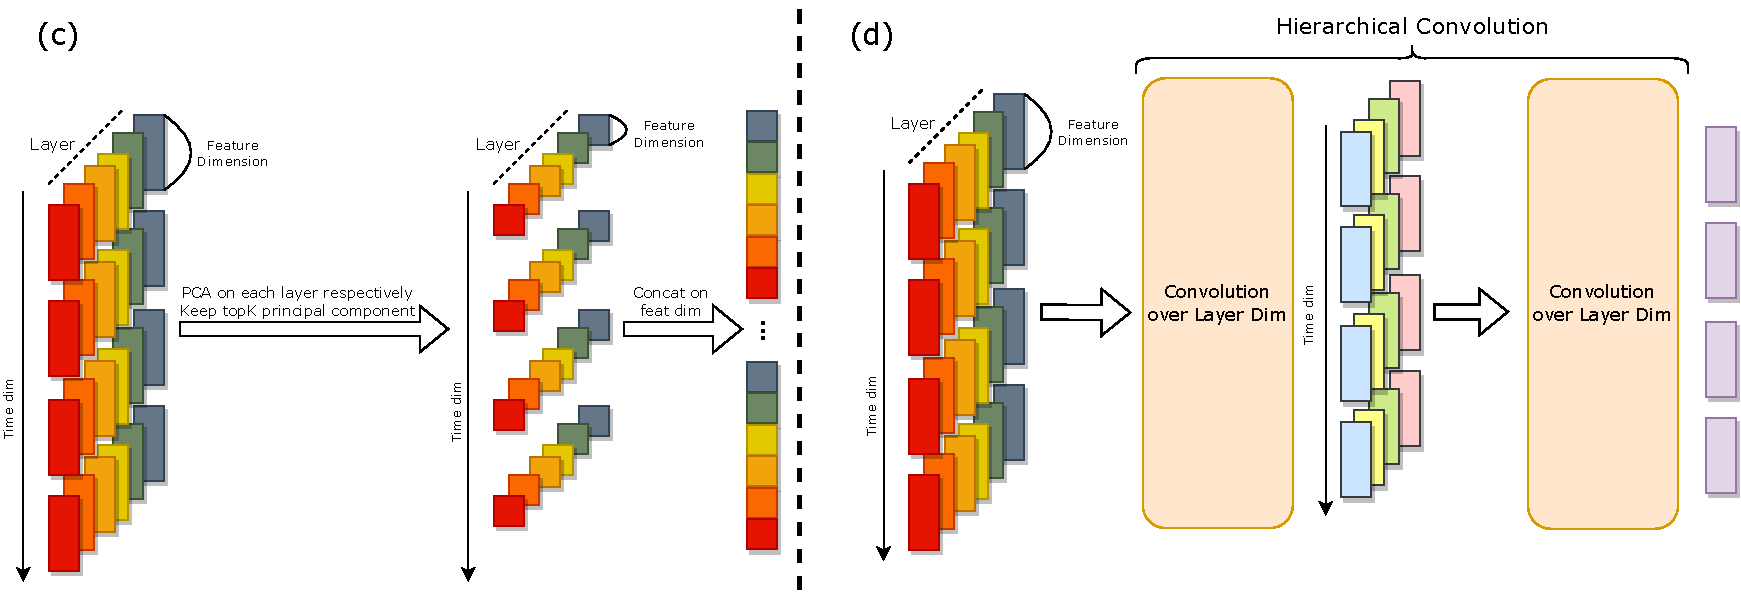
\includegraphics[width=\linewidth]{figs/interface_cd.pdf}
%     \caption{Proposed interface designs. (a): Multiple Groups of Weighted Sum (2 Groups for example), (b) Concat + Learnable Projection, (c) PCA dimension reduction + Concat, (d) Hierarchical Convolution over layer dimension}
%     \label{fig:interface}
% \end{figure}

\subsection{Proposed Interfaces}

\subsubsection{Grouped Weighted Sums}
An intuitive way to reduce the information collision of a single weighted sum is instead to use multiple weighted sums, each of which only has access to a subset of the upstream layers.
Specifically, after conducting a weighted sum within each subset of upstream layers, we concat the results of each group along the feature dimension.
Then we use a learnable projection to project the feature dimension to that of the downstream model.


% We first split the upstream model layers into $K$ groups, $\boldsymbol{h}=\mathrm{Concat} \left[ \boldsymbol{G}_0 \cdots \boldsymbol{G}_{K-1}  \right]$.
% Within each group $\boldsymbol{G}_{k}$, we apply weighted sum $\boldsymbol{p}_{k}=\sum_{}^{\left| \boldsymbol{G}_k \right|}{{w}_{k,l}\cdot \mathbf{G}_l}$, where ${w}_{k,l}$ is the learnable weight for $l$ layer of group $k$, .
% Finally, we concatenate the $\boldsymbol{p}_{k}$ vectors together along the feature dimension and use a learnable projection to project the feature dimension to that of the downstream model.
% \begin{equation}
%     \mathrm{I}_{\mathrm{MultiWS}}\left( \boldsymbol{h}  \right)=\mathrm{Proj}\left( \mathrm{Concat} \left[ \boldsymbol{p}_{1}; \boldsymbol{p}_{2} ; \cdots ; \boldsymbol{p}_{k} \right] \right)
%     \label{eq:multiWS}
% \end{equation}


\subsubsection{Concatenation + Learnable Projection}

Another type of interface concatenates all layer representations $\boldsymbol{h}$ along the feature dimension and uses a learnable projection layer to automatically decide the features that are beneficial to the downstream model. 
Specifically, we reshape $\boldsymbol{h}$ from $\left( L,T,D \right)$ to $\left( T,L\times D \right)$,
then 
% use a learnable projection matrix to
project $\left( T,L\times D \right)$ back to the original upstream model dimension $\left( T, D \right)$.

% \subsubsection{Learnable Layer-wise Projections + Weighted Sum}

% Another interface method aimed at reducing the information collision when performing a weighted sum over layers, we add a learnable linear projection for each layer representation before applying the conventional weighted sum aggregation.
% Ideally, the linear layers can learn to rotate and scale information in each layer to different dimensions.

\subsubsection{Hierarchical Convolution over Layers}

Even though the feature manifold differs among each layer of the upstream model, neighboring layers can still possess similar feature distributions due to the residual connection in the transformer layers~\cite{vaswani2017attention}.
Motivated by the local structure of the hidden representation across the layer dimension, we apply 1D convolutions over the layer dimension to aggregate the information across layers.
In practice, an interface design should be adaptable to upstream models with an arbitrary number of layers.
Hence, in our paper, we fix the kernel size=$5$, stride=$3$ for our convolution layer and we stack $\lfloor \mathrm{log}_3{L} \rfloor$ identical convolutional layers, which has the effect of collapsing the output of all models layers down to a single vector at the output of the convolutional stack (as shown in Fig.~\ref{fig:interface_conv_cls} (a)).
We leave further convolutional hyperparameter optimization for future study.

\subsubsection{CLS Pooling over layer dimension}

We can use an attention module to aggregate information across layers rather than using convolutions.
% Instead of using convolutions across layers, we can use an attention module to aggregate information across layers.
Specifically, at each timestep we view all the layers of the upstream model as a sequence of tokens and concatenate a learnable CLS vector~\cite{devlin-etal-2019-bert} to this sequence. A Transformer layer is then used to aggregate information across all layers at the same time step into the CLS token (as shown in Fig.~\ref{fig:interface_conv_cls} (b)). 
% Specifically, we add a learnable CLS vector to the output of the upstream model, and add a Transformer layer which enables the CLS vector to aggregate information across all layers in the model (as shown in Fig.~\ref{fig:interface_conv_cls} (b)).
A key difference compared to our other proposed interface designs is that CLS Pooling is data-dependent, while other methods are only task-dependent. 
% \david{Ian can you say some more details here? Is each upstream layer treated as a single token?}

\subsubsection{PCA + Concatenation}

Besides the above parametric methods, we also investigated layer-wise dimensionality reduction via Principal Component Analysis~(PCA), followed by concatenation across layers. Using the HuBERT Base model as an example upstream model, we take only the top 60 principal components of each Transformer layer and concatenate them together, resulting in $60\times 13=780 \approx768$ dimensions, which is roughly the same as the upstream model feature dimension. 
% \david{Ian can you say something about how the PCA transform is learned}
Practically, the PCA transform is learned from each downstream task dataset respectively.

